\chapter{Results}
\label{chap:results}

In this chapter we will present our results from analyzing the data in the blockchain using the methods described in \cref{chap:metodology}. 
Bitcoin has a testnet used for development and testing of experimental functionality, which the LN have been tested on for longer than it has been used on the mainnet. We have used both the testnet and the mainnet in the project; our reasoning for this is the LN on the testnet is larger, and people are testing a wide array of use cases and functionality, using testnet coins without any value; on the mainnet users have Bitcoin with value, perhaps resulting in more realistic user behaviour which could impacts the data generated.
By using both Bitcoin networks we will have both edge cases and cases accurately reflecting normal user behaviour.
The testnet has its own blockchain which is publicly available in the same manner as the mainnet blockchian. Collecting data from the LN as discussed in \cref{sec:ln_analysis} was done in two intervals of one week each.
Creating a snapshot of the LN state on each block for a week results in around 1000 blocks worth of data. This should be sufficient to verify our methods of identifying relevant LN transactions, and doing this twice allowed us to make adjustments after the results of the first interval. 

\section{Method verification with LN data}
\label{sec:method_verification}

Comparing data from the LN with our data from the blockchain, provided us with results about the extent our identification methods is able to identify LN channels on the blockchain. There was three sets of data was used in these comparisons: 
\begin{itemize}
    \item The set \( \alpha \) , containing channels from the LN closed during the capture interval. 
    \item The set \( \beta \), containing channels from the blockchain identified using timelocked redeem scripts,
    \item The set  \( \gamma \), containing potential channels identified on the blockchain using 2of2 multisig scripts.
\end{itemize}

As we stated previously a LN channel uses the {\tt P2WSH} 2of2 multisig type for the on chain founding - closing output - input pair. In \cref{detection_ms} we discussed how this could be used to give us a set of potential transactions being related to LN channels. Because the on-chain channel transactions must be of this type the \( \gamma \) set is guaranteed to include all channels closed in the block interval used for the search. It also means that the two other sets will be subset of \( \gamma \). So the relations between the sets should be as follows:

\begin{equation} \label{eq:1}
      \alpha \subseteq \gamma, \hspace{10pt} \beta \subseteq \gamma, \hspace{10pt} \beta \subseteq \alpha  
\end{equation}

The two first relations is explained above and is always true for the systems in its current case. The last relation however, will not hold with our data, but ideally it should be true. For this to be the case our method with timelocked redeem scripts for identifying channels should not have any false positives-i.e., identify channels which is unrelated to the LN. Additionally we should also be able to discover all closed channels in our interaction with the LN during the interval, meaning we would get the complete set of channels-i.e., \( \gamma \) contain all LN channels closed in the interval. While the timelocked scripts are very unique and therefore good for identifying channels, and theoretically one could get all LN channels by connection to the LN, this would only be true in a ideal world scenario. So as we will see with our data \( \beta \not\subseteq \alpha \), but keeping the relation in mind will be useful when analyzing the data.

\subsection{First Interval}

\begin{figure}[ht]
    \centering
    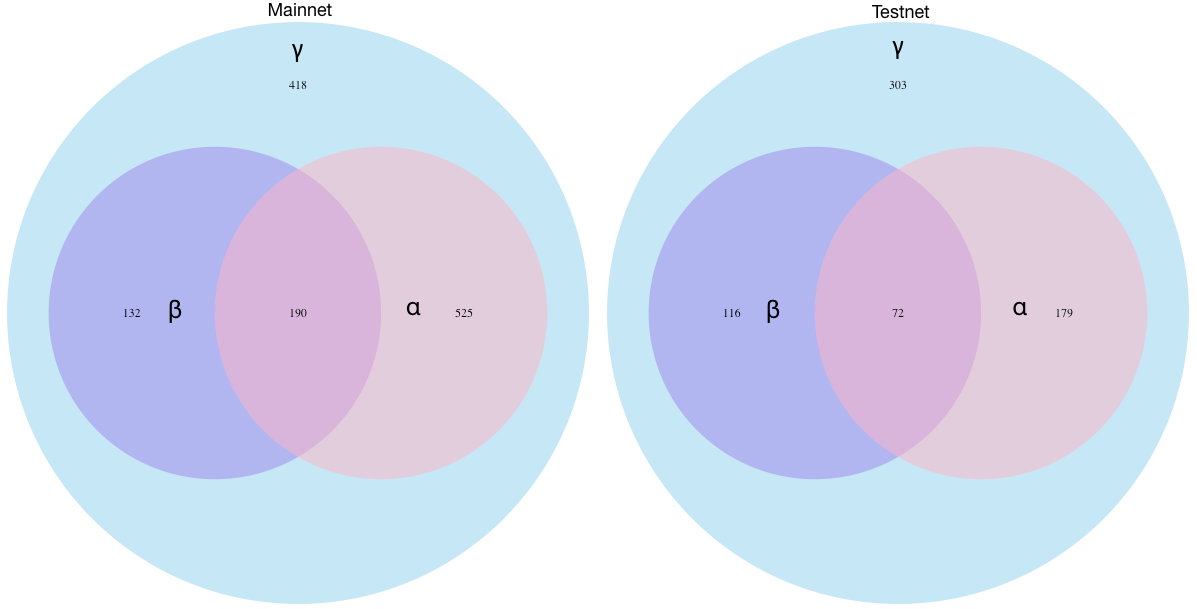
\includegraphics[width=16cm]{figures/graphs/venn_full.png}
    \caption{Venn diagram of channel sets in interval one}
    \label{fig:venn_run1}
\end{figure}

The first collection interval on the mainnet had a length of 1151 blocks, found between block 517855 and 519005. Our modified LND implementation described in \cref{sec:ln_analysis} collected data from the LN and produced the set $\alpha$ containing 715 channels which were closed during this interval. The same interval on the blockchain was parsed two times, once identifying channels using timelocked redeem scripts, and a second time getting all potential channels using multisig identification. This resulted in a $\beta$ set containing 322 channels and a $\gamma$ set with 1265 channels shown on the left in \cref{fig:venn_run1} as a venn diagram. We can see how both $\beta$ and $\alpha$ is a subset of $\gamma$, but $\beta \not\subseteq \alpha$. The intersection $\beta \cap \alpha$ is the number of channels we identified using the timelocked redeem script which where also found trough the LN node. On the mainnet this intersection was 190 which is 36\% of the total channels in $\alpha$. This is reasonable, as the method will only discover a channel if it has been unilaterally closed as we explained in \cref{sec:bc_analysis}, and not if a channel is closed cooperatively which likely will happen more frequently. Taking the ideal world scenario $\beta \subseteq \alpha$ discussed above, into account for this data, we have a large $\beta \backslash{} \alpha$ relative compliment of $\alpha$ in $\beta$ of 132, which is 40\% of the channels in $\beta$. Having a false positive this high is very unlikely because the uniqueness of the timelocked redeem scripts, so we made the assumption that these are actually LN channels which we have not been able to capture in our interaction with the LN. The reason we made this assumption was that it is more likely that not every channel is propagated successfully to our single LN node, than there being instances of timelocked redeem scripts unrelated to the LN on the blockchain. Addiontally, as we explained in \cref{sec:ln_analysis} at least every node running the LND implementation will prune their LN graph of "zombie" channels regularly, so these will eventually no longer be propagated trough the network. This means even if our node does not prune its graph of the network, the channel will never be received in the first place. These are the likely causes of our timelocked channels not being found in the LN channel set.
Taking this into account and assuming the union $\alpha \cup \beta$ are all LN channels, the total number of LN channels closed in this interval would be 847. This would entail that 67\% of 2of2 multisig transactions in our interval is lightning channels. 
\\

For the testnet our LND node collected 838 snapshots starting on block 1290011 and ending on block 1289174. The results are very similar to the mainnet, with the intersection $\beta \cap \alpha$ being 27\% of $\alpah$,
and the $\beta \backslash{} \alpha$ relative compliment of $\alpha$ in $\beta$ being 62\% of channels in $\beta$.
Again, assuming the union $\alpha \cup \beta$ are all LN channels, 55\% of 2of2 multisig transactions is lightning channels. This is however not a upper limit, as our $\alpha \cup \beta$ union is the channels unilaterally closed on the blockchain and channels that have been propagated to our node in the LN. As we discussed our LN node might not be able to get all channels, so there should also be channels not closed unilaterally and therefore not discovered on the blockchain, which we similarly have not been able to collect trough the LN. 
Which would make the total channel count higher, and more of the 2of2 multisig transactions being channels, than is indicted in our results for both the networks.

\subsection{Second Interval}


For our second interval we only collected data from the mainnet, but tweaking the collection slightly compared to interval one. Instead of only peering with the one assigned when starting the node software we added more, up to a total of 10 peers for the duration of the interval. We also ran the node for a few days before starting the collection, so the node would have opportunity to synchronize as much as possible, and perhaps get channels that would have been pruned in that timeframe and not announced to the node at a later time. A total of 1151 snapshots of the LN was created, giving $\alpha$ 446 closed channels. The timelocked identification on the blockchain found  168 channels for $\beta$, while the multisig identification resulted in 667 channels for $\gamma$. For this interval the the intersection $\beta \cap \alpha$ was 26\% of $\alpha$, which is similar to the first interval, with 36\% and 27\% for the mainnet and testnet respectively. However, the $\beta \backslash{} \alpha$ relative compliment of $\alpha$ in $\beta$, was 30\% of channels in $\beta$, compared to 42\% and 63\% in the first interval. Also, if the union $\alpha \cup \beta$ all is LN channels, it would entail 75\% of the 2of2 multisig transactions are lightning channels. This would indicate we have been able to collect more channels from the LN, which the size of $\apha$ compared to $\gamma$ also shows: in this interval $\alpha$ is 67\% of $\gamma$, while in the first interval this were between 55-56\% for both networks. This supports our suggestion made in the previous subsection about there being a number of channels which we are unable to collect trough the LN, but ensuring that the collection node can synchronize as much as possible is important.
This would also mean that than 75\% of 2of2 multisig transaction are likely LN channels. 

\begin{figure}[ht]
    \centering
    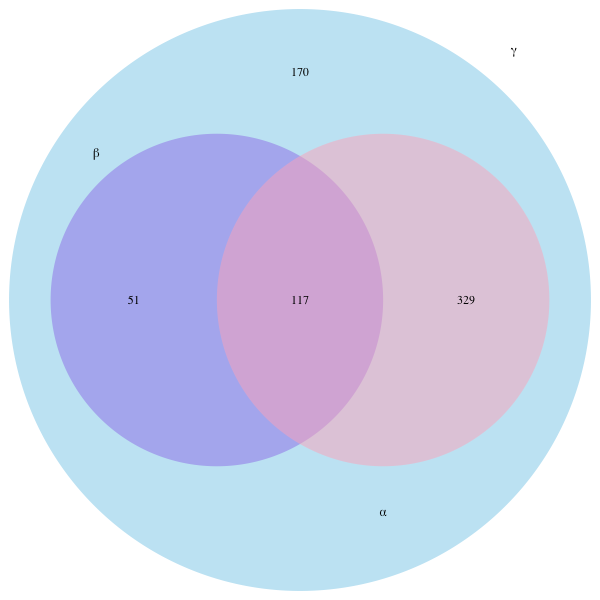
\includegraphics[width=10cm]{figures/graphs/venn_run2.png}
    \caption{Venn diagram of channel sets during interval two}
    \label{fig:venn_run2}
\end{figure}

\section{Lightning Network size}

We mentioned in \cref{subsec:information_ln}, how we could use the fact that the outputs used for creating a channel has to be of the {\tt P2WSH} type, to determine the maximum possible size of the LN.
While parsing the blockchain we have counted all unspent {\tt P2WSH} outputs for each block height, in both the mainnet and the testnet.
The results of this can be found in \cref{fig:ln_size}, as a graph showing unspent {\tt P2WSH} outputs for different block heights.
We can see a distinct difference between the two networks: the mainnet has a more organic growth as a result of real world use, while the testnet graph is characterized by the testing which the network is used for. The sharp decline in unspent outputs on the mainnet at around block 505 000 can be explained by the sharp decline in fees for doing transactions at that time \cite{mempool_stats}, which incentivized users to consolidate their unspent outputs into fewer bigger ones. 

\begin{figure}[ht]
    \centering
    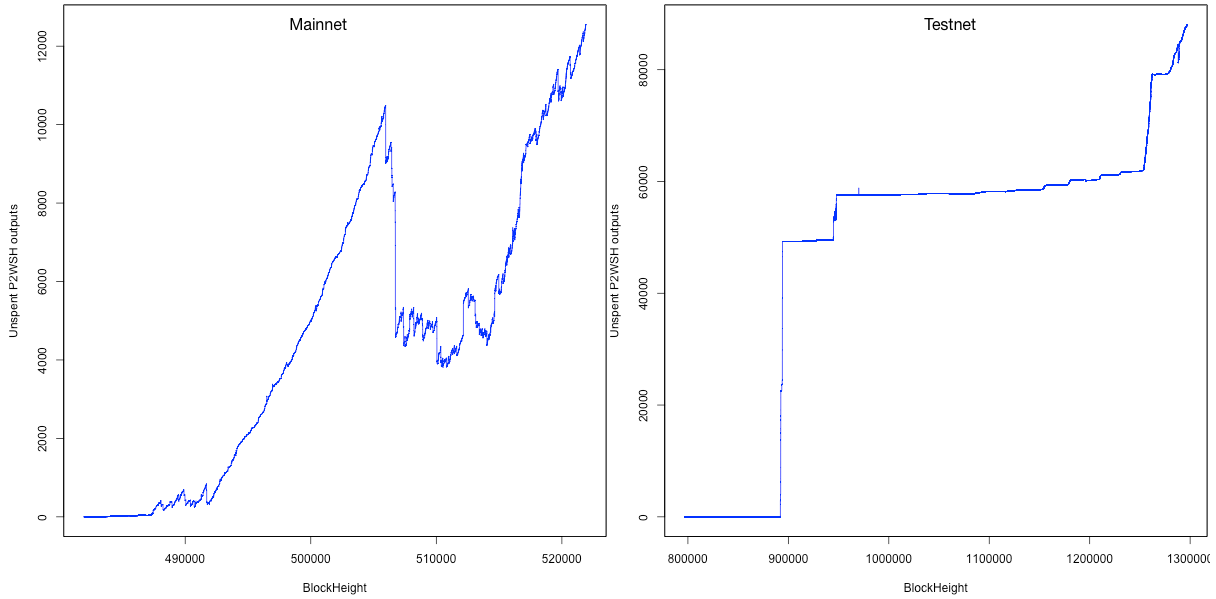
\includegraphics[width=15cm]{figures/graphs/ln_size_bc.png}
    \caption{Maximum size of the LN based on unspent P2WSH outputs on the blockchain}
    \label{fig:ln_size}
\end{figure}

\begin{figure}[ht]
    \centering
    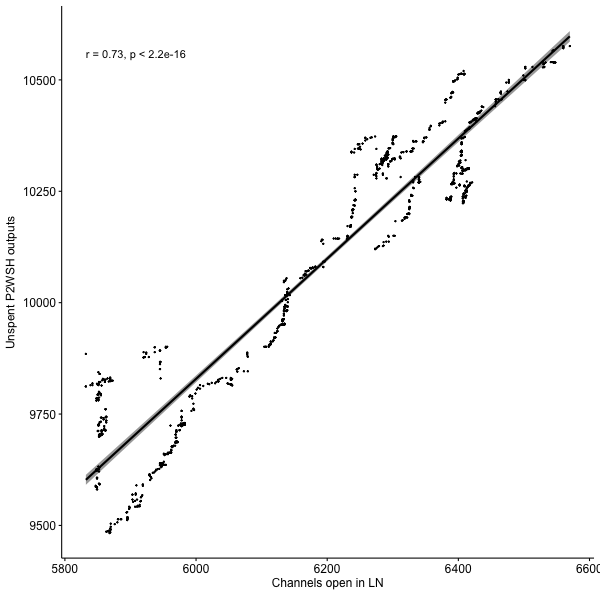
\includegraphics[width=10cm]{figures/graphs/channel_p2wsh_correlation_mainnnet.png}
    \caption{Correlation between unspent P2WSH outputs and channels open in the LN mainnet}
    \label{fig:correlation}
\end{figure}

\begin{figure}[h]
    \centering
    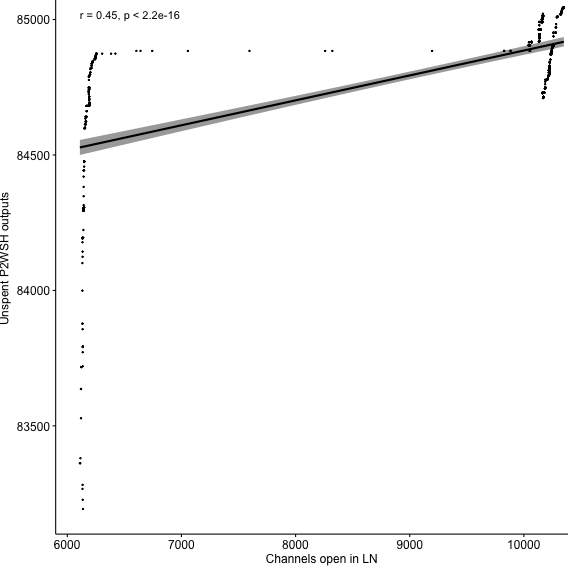
\includegraphics[width=10cm]{figures/graphs/channel_p2wsh_correlation_testnet.png}
    \caption{Correlation between unspent P2WSH outputs and LN channels on the testnet}
    \label{fig:correlation_testnet}
\end{figure}

While the unspent output count provides a concrete upper limit on the number of channels and therefore size of the LN, we also wanted to know to which degree the amount of unspent {\tt P2WSH} transactions was correlated to the size of the LN. It is clear that changes in the size of the LN will impact the number of {\tt P2WSH} outputs/inputs, but there might be many other transactions not related to the LN having a larger impact. From the data we collected from the LN itself we constructed a total channel count for each block height in the collection interval. Similarly we isolated the same block interval with the {\tt P2WSH} output count from the blockchain. These two variables allowed us to compare the changes of number of channels in the LN and number of unspent {\tt P2WSH} outputs. We used Kendall rank correlation coefficient on this data for the mainnet, which gave us a correlation coefficient of 0.73 indicating a strong positive correlation. The scatter plot for this can be seen in \cref{fig:correlation}.
We did the same for the interval of testnet data we collected, which resulted in a coefficient of 0.45 which is only a moderate correlation. 
The scatter plot for the testnet can be seen in \cref{fig:correlation_testnet}.
Both tests has the same p value: p < 2.2e-16. 
While the two things will be correlated naturally due to the need for channel outputs to be {\tt P2WSH}, the results here indicate there is a strong correlation. The testnet showing a weaker correlation can be due to the unnatural use taking place on the testnet, as was apparent from \cref{fig:ln_size} graph showing unspent output for different block heights. Additionally, the correlation was limited to the amount of data from our collection intervals, meaning we could only correlate the two for around 1000 blocks.

\section{Stats from complete runs}
\label{sec:fullrun}

We also tried to run our software with the timelocked redeem scripts method for as long as there was any {\tt P2WSH} transactions on the blockchain, to collect as many channels as possible. As this method is precise and can find a fair amount of channels, it was chosen as the main method when doing this. This resulted in a set of channel graphs for every unilaterally closed channel that has existed up to the point we started parsing. On the mainnet we started on block 524 816 and ended on block 464 816 resulting in a total of 3 809 channels found. For each timelocked redeem script we also checked how the script was evaluated, telling us if the revocation or timelocked clause were used. On the mainnet we found that 163 timelocked outputs were spent with the revocation key, meaning at least this many old commitment transactions was published. In \cref{timelocked_identification} we described how users could spend unconfirmed transactions, resulting in the transactions being found within the same bock. We found a total of 29 such instances, only checking the transactions wihin our channel graphs.
Regarding HTLC frequency on-chain, we found a total of 163 transactions containing HTLC redeem scripts. 101 of these turned out to be spending outputs from closing transactions of graphs we already had identified, which means we could have identified 62 more channels by also using this method.
Doing the same for the testnet resulted in 8047 channels found, starting on block 1 316 196, and ending on block 816 196. Here we found 38 timelocked outputs spent with the revocation key, and 430 of our transactions being found within the same block. On the testnet we found 566 HTLC transactions, with 143 of them not being connected to any of the channel graphs we had identified. 
Using these two sets of channel graphs, we extracted stats about the channels as discussed in \cref{subsec:information_ln}. This gave us  data on the value used in each channel as the amount of Bitcoin (btc), and the lifetime of channels in terms of the number of blocks between opening and closing the channel. The results of this can be seen in \cref{subgraph_stats}.
We also included the same stats from the data collected from the LN during our intervals described in \cref{sec:method_verification}. 
While this can provide some comparison between the stats, as found on the blockchain and from the LN, it will has limits as the blockchian data is for a much longer time interval compared to the LN data.
The One clear difference between the mainnet and testnet is the amount of value used for the channels, as we briefly mentioned before coins on the testnet has no value to people, so it would be natural that they are more liberal when creating channels there. We can also see that the testnet data is similar for both theblockchain and LN, while this is not the case for the mainnet. This can indicate that the these stats on the testnet are more constant, while the mainnet channels now has lower value but higher lifetime than the average for all time.
\\

\begin{table}[ht]
\centering
\caption{Value and lifetime for channels}
\label{subgraph_stats}
\begin{tabular}{l|c|c|c|c}
%\hline
                                              & \textbf{Mainnet} & \textbf{LN Mainnet}& \textbf{Testnet} & \textbf{LN testnet} \\ \hline
\textbf{Sample size (channels)}              & 3809             & 715           & 8047                     & 251            \\ \hline
\textbf{Average Channel value}               & 0.00439556     & 0.0023375        & 0.07086336            & 0.07758942       \\ \hline
\textbf{Median channel value}                & 0.001         & 0.0005             & 0.005            & 0.06        \\ \hline
\textbf{Standard Deviation Channel value}    & 0.01384113       & 0.00586706      & 0.07067473            & 0.07191958        \\ \hline
\textbf{Average channel lifetime}            & 1 600            & 1 940           & 2 441                & 1 269            \\ \hline
\textbf{Median channel lifetime }             & 693              & 1 836             & 433                  & 312              \\ \hline
\textbf{Standard Deviation channel lifetime} & 2 183            & 1 791           & 5 631                & 4 059            \\ \hline
\end{tabular}
\end{table}

In \cref{channel_input_output} we see the distribution for the number of inputs and outputs to channels. These results are fairy similar for both networks, we should however note the percent of channels having two outputs in relation to the percent having only one input. For the mainnet the percent of channels having one input is 70\%, and the percent of channels only having one output is 71\%. As discussed in \cref{subsec:information_ln} we cannot easily match input - output pairs to users in the channel, so these number either means that many channels does no off-chain transactions at all, meaning the single input will be outputted back to owner, or that all founds in the channel ends up at one of the entities as a result of off-chain transactions. In the testnet column we can see how the single output percentage is lower compared to the single input percent, also the double output percent is higher than the double input. This indicates that many single founded channels ends up with splitting the value when they close, and as we stated in \cref{sec:bc_analysis} this enables us to say that off-chain transactions has taken place inside the channel.
This difference is also present when we checked how many channels had the same number of inputs as outputs. On the mainnet 57\% of channels found have the same number of inputs as outputs, while on the testnet this is 46\%. 
Using the HTLC transactions we found which also was outputs from closing transactions in our channel graphs, we can determine how often they occur: 2.6\% of channels on the mainnet and 5.2\% on the testnet would have one HTLC output. Comparing with the \cref{channel_input_output} we can see how this can make up all of the channels with two outputs, and also the ones with three or more as channels certainly can have more HTLC outputs.
\\

\begin{table}[ht]
\centering
\caption{Percentages of input - output count for channels}
\label{channel_input_output}
\begin{tabular}{l|c|c}
%\hline
                                                                      & \textbf{Mainnet} & \textbf{Testnet} \\ \hline
\textbf{Channels with one input}             & 69.3            & 76.4            \\ \hline
\textbf{Channels with two inputs}            & 23.2            & 16.8            \\ \hline
\textbf{Channels with three inputs}          & 4.5             & 3.8             \\ \hline
\textbf{Channels with more than three inputs} & 2.8             & 2.9             \\ \hline
\textbf{Channels with one output}             & 69.2            & 50.5            \\ \hline
\textbf{Channels with two outputs}             & 29.6            & 46.3            \\ \hline
\textbf{Channels with three outputs}            & 0.8             & 2.1             \\ \hline
\textbf{Channels with more than three outputs} & 0.2             & 0.8             \\ \hline
\end{tabular}
\end{table}

\section{Linking}

Our software also linked the sets of channels graphs found, using the methods and heuristics described in \cref{sec:linking}.
The linking was done, both on the set of channel graphs found on the blockchain during the LN collection intervals, and the sets of channels found when doing complete runs as described in \cref{sec:fullrun}. In \cref{key_reuse_table} we can see the findings in regards to key reuse, when checking the channels graphs for testnet and mainnet found during the complete runs. Using the 3 809 channels we found on the mainnet, we extracted a total of 26 824 unique keys from the transaction in the graphs, with 1 370 or 5.1\% of these being found multiple times. These keys combined where reused 2 850 times, which if the key reuse was evenly distributed in the channel graphs, each channel graph would have 0.75 keys used in another channel graph. For the 8 047 channels found on the testnet, we got 50 050 unique keys. The results here are very similar to the mainnet, with 6.5\% of the keys found were reused, and 0.9 reused keys per channel graph if they were equally distributed. As discussed in \cref{sec:linking} regarding key reuse: key reuse within the same channel graph does not let us allow to link channels, but our results below does not take this into account, but we will address it later in this section.
\\

\begin{table}[ht]
\centering
\caption{Key reuse in channel graphs found in complete runs}
\label{key_reuse_table}
\begin{tabular}{l|c|c}
%\hline
                                                    & \textbf{Mainnet} & \textbf{Testnet} \\ \hline
\textbf{Unique Keys found}                         & 26 824              & 50 050 \\ \hline
\textbf{Unique keys reused}                        & 1 370               & 3 250 \\ \hline
\textbf{Instances of key reuse}                    & 2 850               & 7 240 \\ \hline
\textbf{Maximum number of reuses for a single key} & 23               & 171 \\ \hline
\textbf{Average reuse of keys}                     & 2                & 2.2  \\ \hline
\end{tabular}
\end{table}

Our two other heuristics was also used on these channel sets, allowing us to determine how many channels we were able to link using these. The results of this is shown in \cref{table:connections}. For heuristic one, were we found directly connected graphs trough outputs - inputs, we have separate results for each possible output which can be the source of such a link. We discovered a clear difference between the different outputs: the outputs from the founding transactions makes up over 65\% of the connections found using heuristic one, both on the testnet and mainnet, compared to 2.1\% or less for the outputs from the closing transactions. The outputs from the timelocked transactions makes up 30\% and 33\% of the connections on the mainent and testnet respectively. One possible explanation for this difference has to do with the value of the outputs: closing and timelocked outputs are used to give one party their value from the channel, meaning the value of these outputs is limited to the channel balance of the participant owning them; outputs from the founding transaction on the other hand, is used to transfer change resulting from the output spent to found the channel, which has no size limit, meaning a output many times the value of the channel can be used. Unless multiple inputs is used to found a channel, creating a new channel using the outputs from another will limit the value of the founding input to the balance in the previous channel. A possible reason for the difference between closing and timelocked outputs could be the recommendation to spend timelocked outputs discussed in \cref{sec:linking}, which means if one is closing many channels unilaterally at the same time, consolidation of all timelocked outputs into one timelocked transaction is a natural thing to do; this would cause graph overlap, but also create a high value output from the timelocked transaction which could be used to found new channels. Heuristic 3 which used graph overlap or multi-input timelocked transactions provided 12\% on mainnet, and 24\% on the testnet, of the total connections found using both heuristic two and three.

\begin{table}[ht]
\centering
\caption{Relations found between channel graphs using heuristic one and two}
\label{table:connections}
\begin{tabular}{l|c|c}
%\hline
                                        & \textbf{Mainnet} & \textbf{Testnet} \\ \hline
\textbf{Total relations found}       & 1586              & 5 715             \\ \hline
\textbf{Founding output relations}   & 931               & 2 824             \\ \hline
\textbf{Closing output relations}    & 30                & 2                \\ \hline
\textbf{Timelocked output realtions} & 435               & 1 499             \\ \hline
\textbf{Graph overlap relations}     & 190               & 1 390             \\ \hline
\end{tabular}
\end{table}

If we combine our results of using all three heuristics on the channel sets, we get a total of 4 436 relations between the channel graphs in the mainnet. This enabled us to crate 2 182 links between channels. The reason this this difference is redundancy for the connections, and key reuse within a single channel graph. This means that 2254 of our relations, or about 50\% where redundant, but only 36 of them being reuse of the same key in the same channel graph. The set of linked channels can be seen visualized in \cref{fig:cg_mainnet_full}, were we have created a channel network as discussed in \cref{sec:linking}. The network consists of 2 324 smaller components, with each node having a average degree of 1.1. While this graph does not distinguish users, we can based on how these components is structured reveal additional information about the users participating in the channels. 
As edges represent at least one common user being present both nodes, we can create the property: for adjacent nodes there can be at most three different users, and minimum two users. This means if the distance between vertices is more than one, we can no longer be sure if if there is common user participation, but we cannot rule it out either. More importantly, it has a impact on complete components-i.e., every node is connected to every other node. Because the property we defined must hold for every node in such a complete component, there are only two possibilities with regard to user participation: there can be at most three total users in the component, or that one user participates in all nodes, but with a different second user in each. 
So either there are three total users in such a component, or the number of nodes plus one total users, because each node has a different user plus the one participating in all.
We can see a few examples of such components in \cref{fig:cg_mainnet_full}, and also some components having a similar structure, but having some additional nodes which is not part of the complete core of the component.
\\

We did the same as discussed in the previous paragraph for the set of channel graphs from the testnet. The total relations using all three herusitcs was 12 955, while the amount of links we could create was 7084. Again 45\% of the connections we found where redundant for actually linking the channels. Here the number of reused keys within a single channel graph was 113, which is relatively small compared to the 5758 other redundant relations.
The channel network shown in \cref{fig:cg_testnet_full} is more connected than the mainnet in \cref{fig:cg_mainnet_full}, with the testnet network having over twice as many nodes, but only having 617 more components. We can see this difference clearly with the large component in the middle of the testnet graph. As the LN is one network, it should consist of one dynamic component, meaning a historic network graph should also ideally have one large component. While we can see this beginning to emerge in our testnet channel network, it is very clear in the channel network constructed using LN data as seen in \cref{fig:channel_network_LN_mainent}.
\\

\begin{figure}[ht]
    \centering
    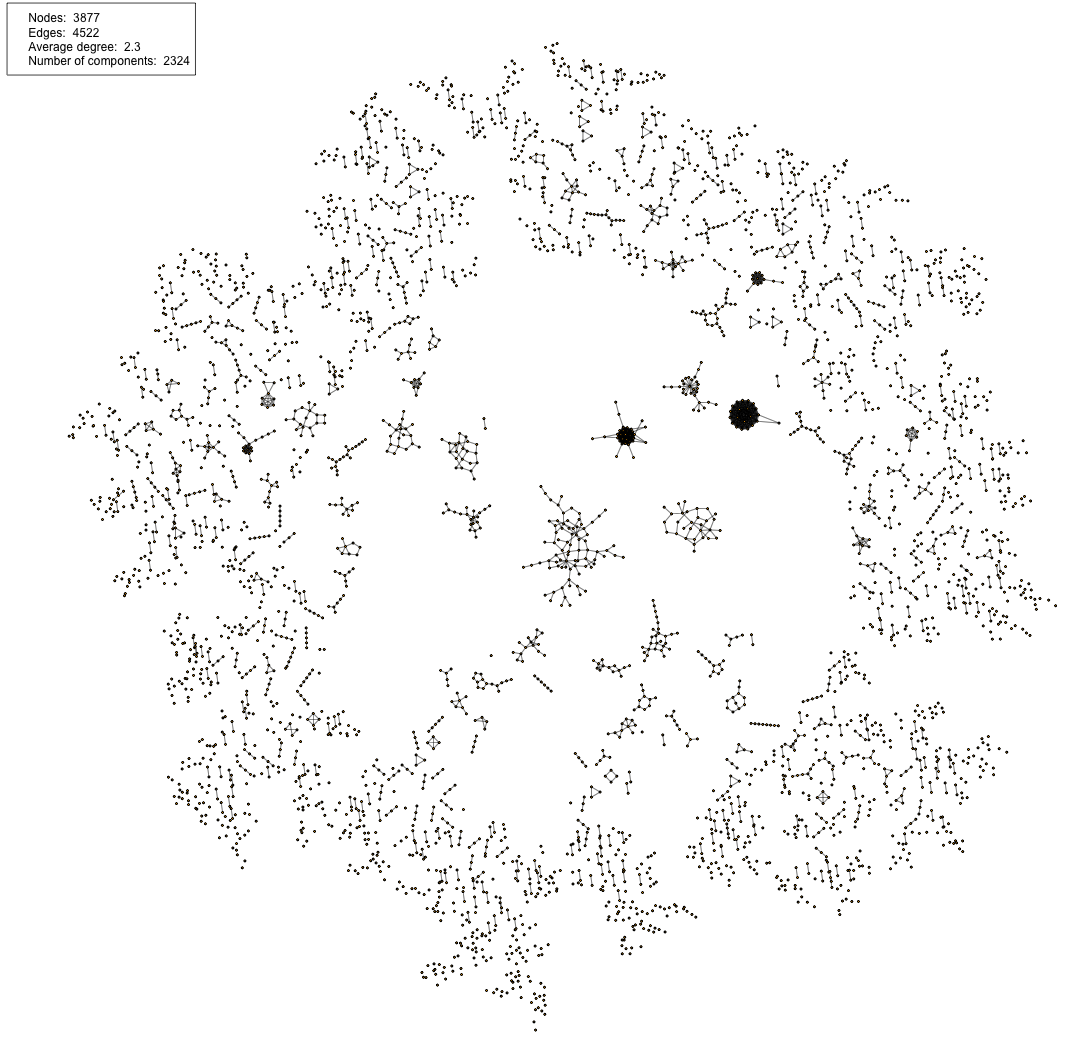
\includegraphics[width=13cm]{figures/graphs/cg_bc_mainnet_full.png}
    \caption{Channel network for mainnet}
    \label{fig:cg_mainnet_full}
\end{figure}

The channel network in \cref{fig:channel_network_LN_mainent} based on LN data from interval 1, was created so we could compare it with the networks we crated by linking blockchain information. This would allow us to see how connected a channel network should ideally be if all relations where available to us in the blockchain. In the LN data we collected during the intervals we used the node id, which identifies a node/user, to link the channels that nodes participated in. While users are easily separable by this id, we ignored this to create the same type of network as we did using the blockchain data, meaning edges only indicate common user participation, not a specified user. 
As shown in \cref{fig:channel_network_LN_mainent} the network is highly connected with the 715 nodes having a average degree of 58. We can see that almost all nodes are a part of the main component, with only having 6 nodes not being connected to it.
\cref{fig:histogram} shows the histogram for the node degrees in this network. In this histogram there is one node that sticks out, it has a degree of over 200, compared to the other highly connected nodes which have a degree of around 150. There is also a high frequency of nodes having a degree between 100 and 150. In \cref{centrality_table} we have taken the top five nodes in terms of degree, and calculated some centrality measures for them. The highest connected node with a degree of 239, has also the highest score in the other measures, it can be seen in \cref{fig:channel_network_LN_mainent} as the red node. For the other nodes there is some variation in the scores, but all five nodes being in the top ten for all nodes in every measure, except node or channel 569069835159470080 colored blue in \cref{fig:channel_network_LN_mainent}. For closeness centrality this node was ranked 31, while scoring high on degree and betweenness centrality. 
Comparing this network to the channel network in \cref{fig:channel_network_BC_mainnet}, which we cratered using the channels identified on the blockchain in the same interval, and linked using our three heuristics, we can see how limited our linking capabilities really are.
Having almost six times as many nodes as edges and a average degree of 0.1, we can see how most channels identified has no relation to others we could find, within such a short interval.
The same networks for the testnet interval and the second interval for mainnet can be found in the \cref{appendix_networks}

\begin{figure}[ht]
    \centering
    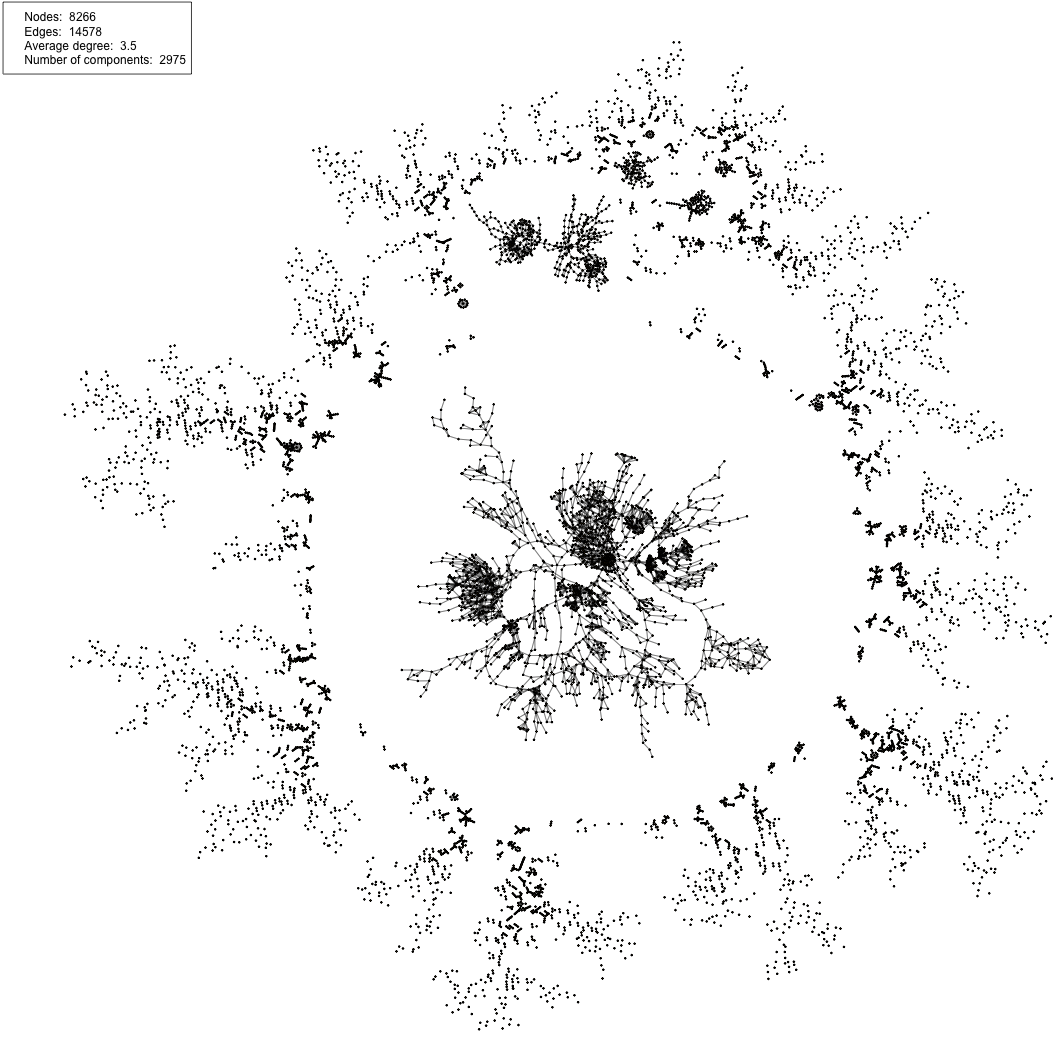
\includegraphics[width=14cm]{figures/graphs/cg_bc_testnet_full.png}
    \caption{Channel network for testnet}
    \label{fig:cg_testnet_full}
\end{figure}

\begin{figure}[ht]
    \centering
    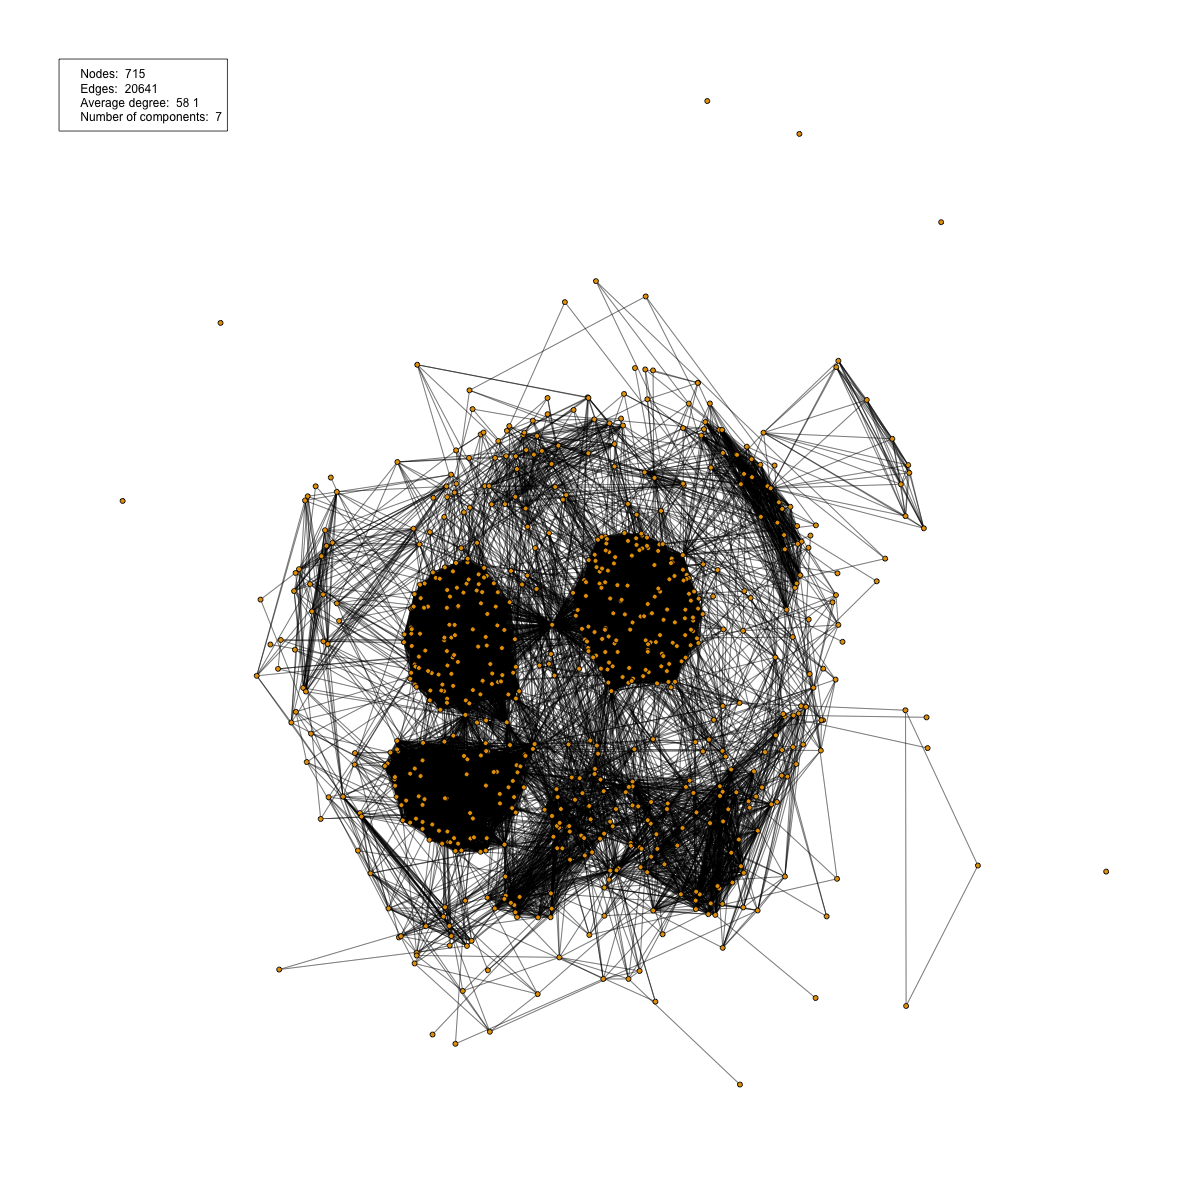
\includegraphics[width=14cm]{figures/graphs/cg_ln_mainnet_run1.png}
    \caption{Linked channels from the LN, mainnet, first interval}
    \label{fig:channel_network_LN_mainent}
\end{figure}

\begin{figure}[ht]
    \centering
    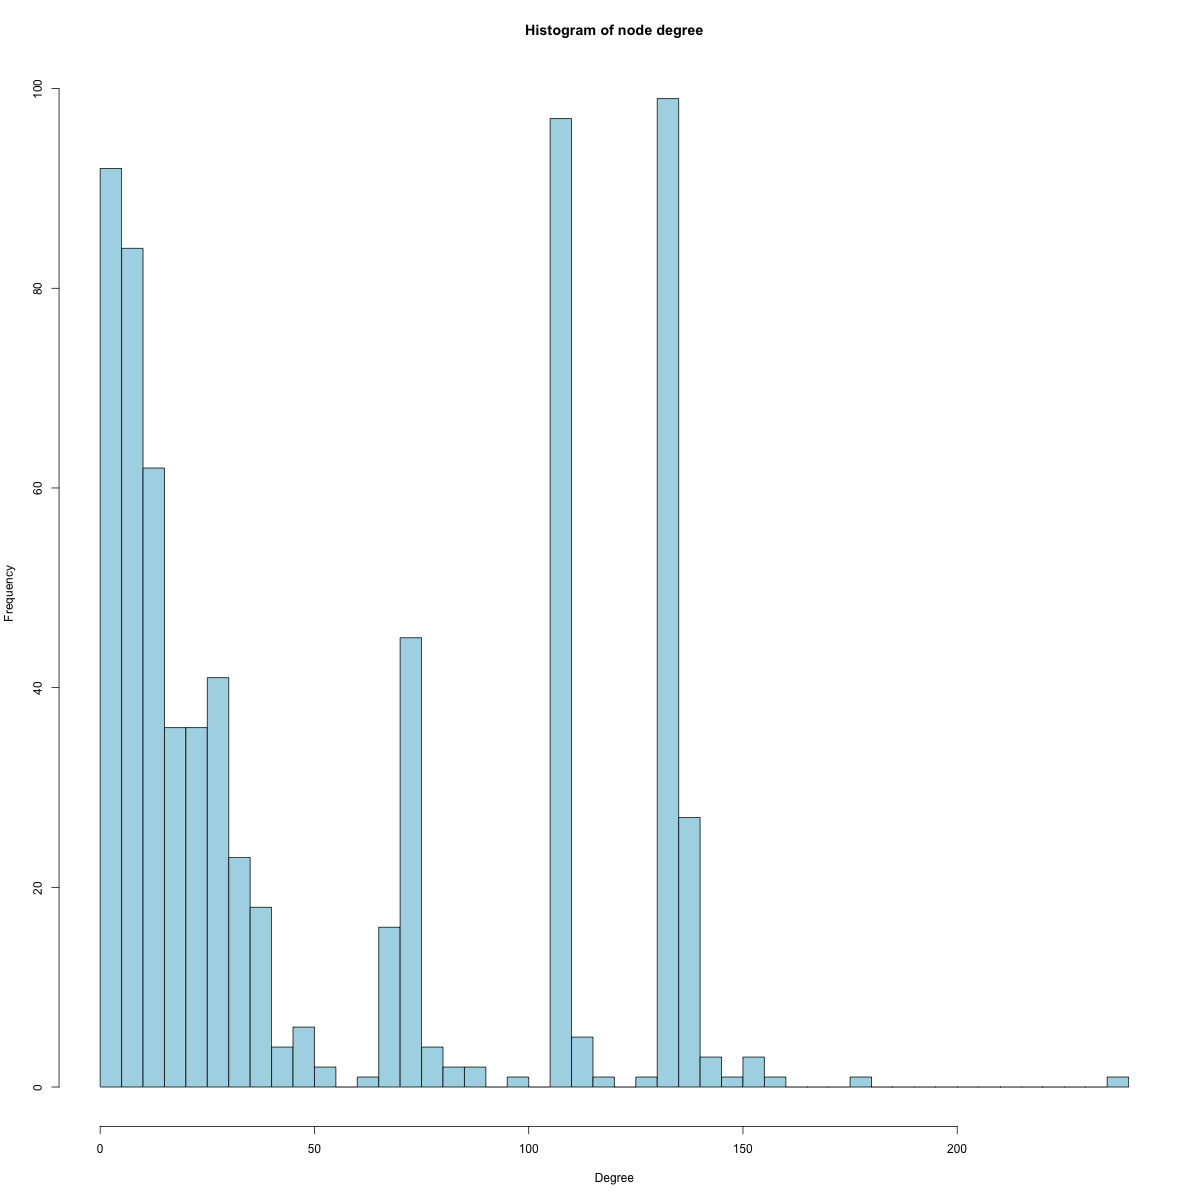
\includegraphics[width=17cm]{figures/graphs/histogram_ln_mainnet_run1.png}
    \caption{Histogram of node degree for the network in \cref{fig:channel_network_LN_mainent}}
    \label{fig:histogram}
\end{figure}

\begin{table}[ht]
\centering
\caption{Centrality measures for the highest degree nodes for the network in \cref{fig:channel_network_LN_mainent}}
\label{centrality_table}
\begin{tabular}{l|c|c|c}
 \textbf{(short) Channel Id}     & \textbf{Degree centrality} & \textbf{Closeness centrality} & \textbf{Betweenness centrality} \\ \hline
\textbf{565863659278368768} &  239 & 0.0001790831 &  23084.374         \\ \hline
\textbf{565758106242187265} &  176 & 0.0001743679 &  10285.468            \\ \hline
\textbf{569069835159470080} &  159 & 0.0001737619 &  11597.068                                 \\ \hline
\textbf{566469490153553920} &  153 & 0.0001763668 &  5733.209                               \\ \hline
\textbf{567496434090377216} &  152 & 0.0001756543 &  6881.286                               \\ \hline
\end{tabular}
\end{table}

\begin{figure}[ht]
    \centering
    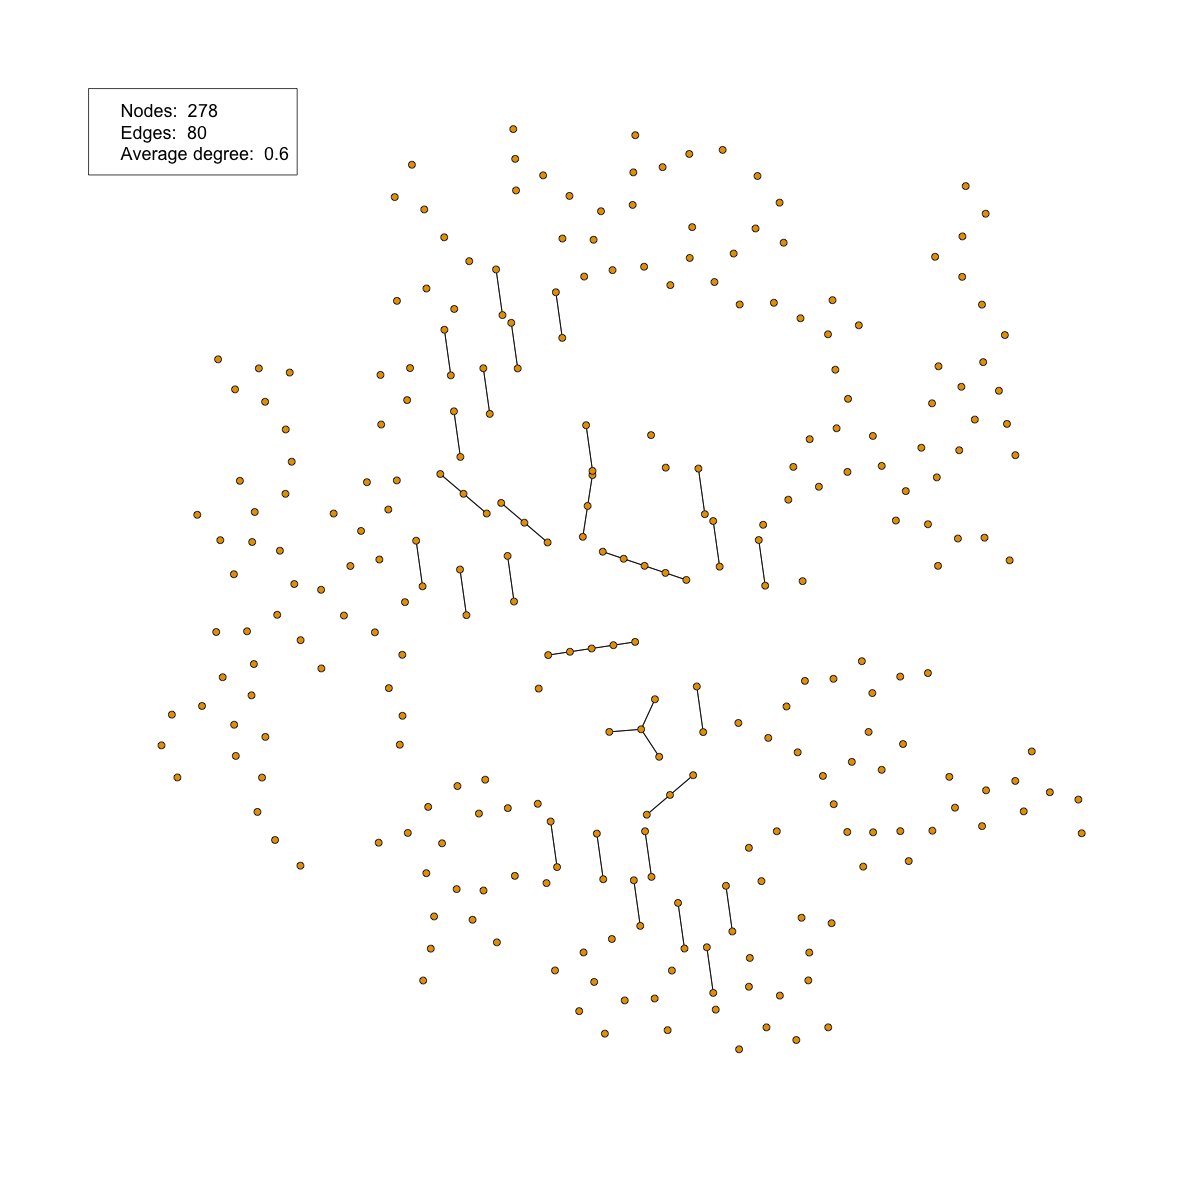
\includegraphics[width=13cm]{figures/graphs/cg_bc_mainnet_run1.png}
    \caption{Linked channels from the blockchain, mainnet, first interval}
    \label{fig:channel_network_BC_mainnet}
\end{figure}
